\begin{task}{1, Vector fields, orbits, and visualization}
For the simulations in this task we use the provided function. Experimental results are used in visualization and analytical results are used to derive types of equilibria.

The plots are obtained using \verb|task1/linear_1_parameter.ipynb|, whereas some plotting utilities are in \verb|task1/linear_plotter.py|. Task 1, 2 and 3 also use \verb|utils.py| for more general plotting utilities.

Firstly, for any eigenvalue it holds that
$$\| A - \lambda I\| = 0$$

for 2x2 matrix
$$(a - \lambda)(d - \lambda) - bc = 0$$
for our matrix $a = b = \alpha$ $c = -4^{-1}$ $d = 0$
$$(\alpha - \lambda)(- \lambda) - (- 4^{-1}\alpha) = 0$$
$$- \alpha\lambda + \lambda^2 + 4^{-1}\alpha = 0$$
whose solutions are
$$(\alpha \pm \sqrt{\alpha^2 - \alpha})2^{-1}$$

Because $dy = -x/4$ the only point where $dy = 0$ has to be $x = 0$. $$dy = 0 \Rightarrow x = 0$$ $$x = 0 \land dx = \alpha y + \alpha x \Rightarrow dx = \alpha y$$ and therefore the only equilibrium for $\alpha \neq 0$ is (0,0). For $\alpha = 0$ points $\{(0,t), t \in R\}$ are equilibria.

At $\alpha = 0$ the equilibria is unstable as if we start at any point that is not an equilibrium we go to positive or negative infinity.

For the other cases we must examine the eigenvalues of A, these are $$(\alpha + \sqrt{\alpha^2-\alpha})2^{-1}, (\alpha - \sqrt{\alpha^2-\alpha})2^{-1}$$.

This has no purely imaginary solutions.
It has real solutions for $\alpha^2 >= \alpha$ so for $\alpha \in R - (0,1)$.
It has imaginary solutions for $\alpha \in (0,1)$. The imaginary part of the two solutions is always complementary.

For $\alpha < 0$ one eigenvalue is positive and the other negative because $$\sqrt{\alpha^2-\alpha} \geq \alpha$$
So for $\alpha < 0$ there will be a saddle at the point (0,0).

The eigenvalues real part is positive or zero for $\alpha > 0$ because 
$$\alpha \geq real(\sqrt{\alpha^2-\alpha}) \geq 0$$
For the $\alpha \geq 1$ this is trivial and because $real(\sqrt{x}) = 0 \ \forall x < 0$ it holds also for $\alpha \in (0,1)$.

If we also take into consideration that the solution is real for $\alpha \geq 1$ that means that there will be an unstable node for this range at the point (0,0).

Since the solution is imaginary for $\alpha \in (0,1)$. The real part is the same for both because $real(\sqrt{x}) = 0 \ \forall x < 0$ and the imaginary parts are complementary to each other because $im(\alpha) = 0$. that means that there will be an unstable focus for this range at the point (0,0).

\begin{figure}[H]
    \centering
    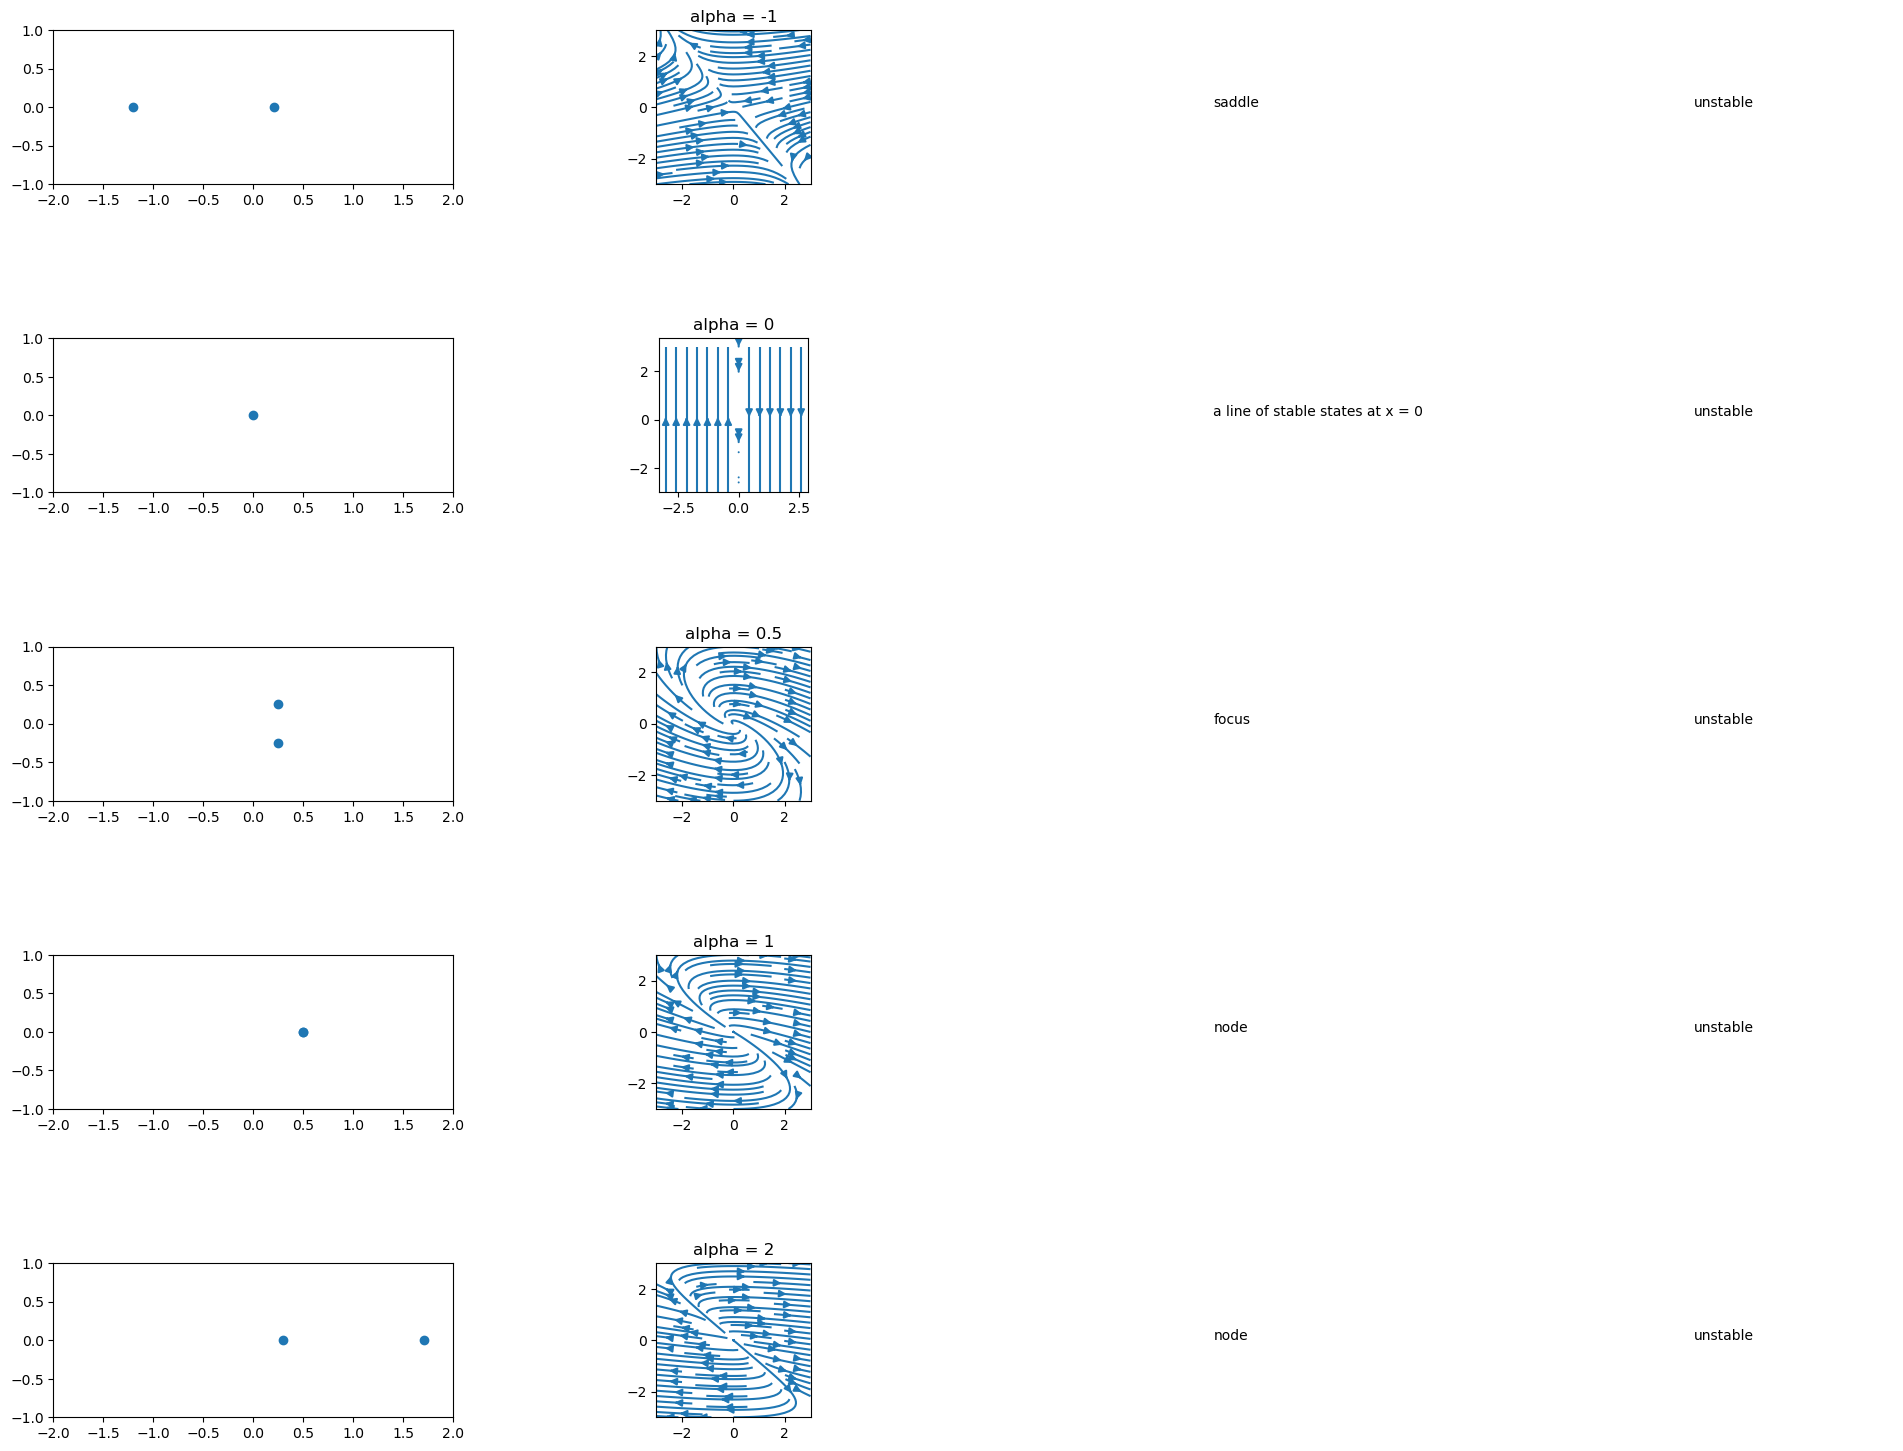
\includegraphics[width=1\textwidth]{images/bfdlinear.png}
    \caption{Phase diagrams of the system $A_\alpha$ at different values of $\alpha$}
    \label{fig:bfdlinear}
\end{figure}

To be able to get all the the types of equilibria (ie. the missing stable node and stable focus) we need to construct a matrix with eigenvalues with negative real parts. Imaginary eigenvalues at some $\alpha$ and real eigenvalues at other $\alpha$.

$B_\alpha$ = $$\begin{bmatrix}
-\alpha & -\alpha\\
\frac{1}{4} & 0
\end{bmatrix}$$

For $\alpha = 0$ there will once again be a line of stable states at $\alpha = 0$ and all other points will go toward negative or positive infinity in the second dimension and keep their first dimension.

For such a matrix's eigenvalues at other values of $\alpha$ a similar equation holds as for $A_\alpha$.
$$\alpha\lambda + \lambda^2 + 4^{-1}\alpha = 0$$
$$(-\alpha - \sqrt{\alpha^2-\alpha})2^{-1}, (-\alpha + \sqrt{\alpha^2-\alpha})2^{-1}$$

For $\alpha \in (0,1)$ the result will be two complementary imaginary values with negative real part so so there will be an attractive focus equilibrium.
For $\alpha > 1$ the result will be two negative values so so there will be an attractive node equilibrium.
For $\alpha < 1$ the result will be one negative and one positive value so there will be a saddle equilibrium.


\begin{figure}[H]
    \centering
    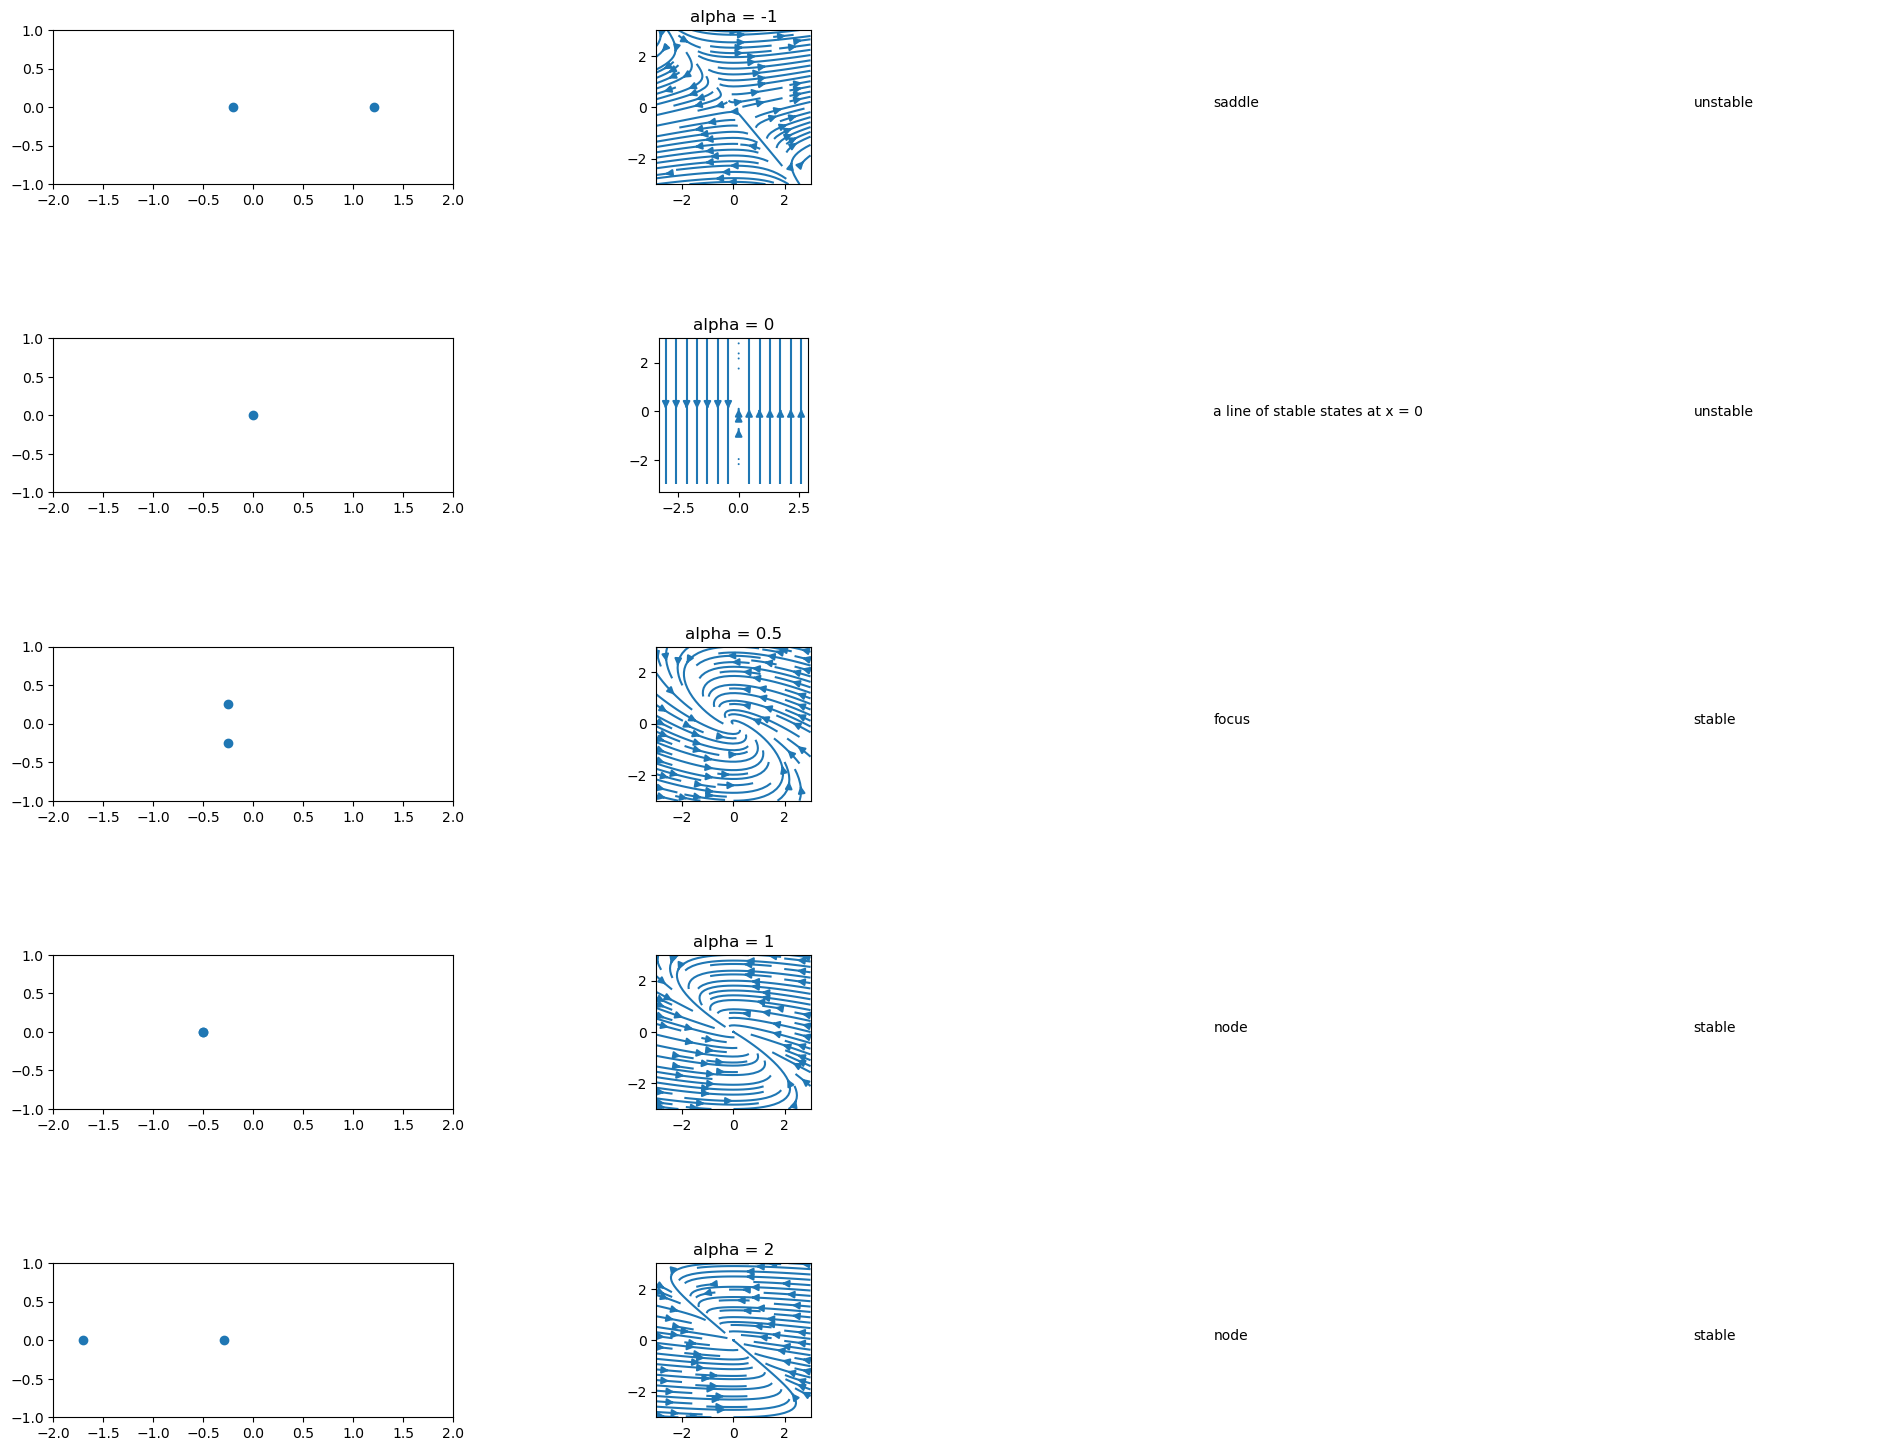
\includegraphics[width=1\textwidth]{images/bfdlinear2.png}
    \caption{Phase diagrams of the system $B_\alpha$ at different values of $\alpha$}
    \label{fig:bfdlinear2}
\end{figure}

And finally we can use these systems to reconstruct the figure from Kuznetsov \ref{Topological classification}.

\begin{figure}[H]
\centering
\subfigure[using $B_\alpha$]{
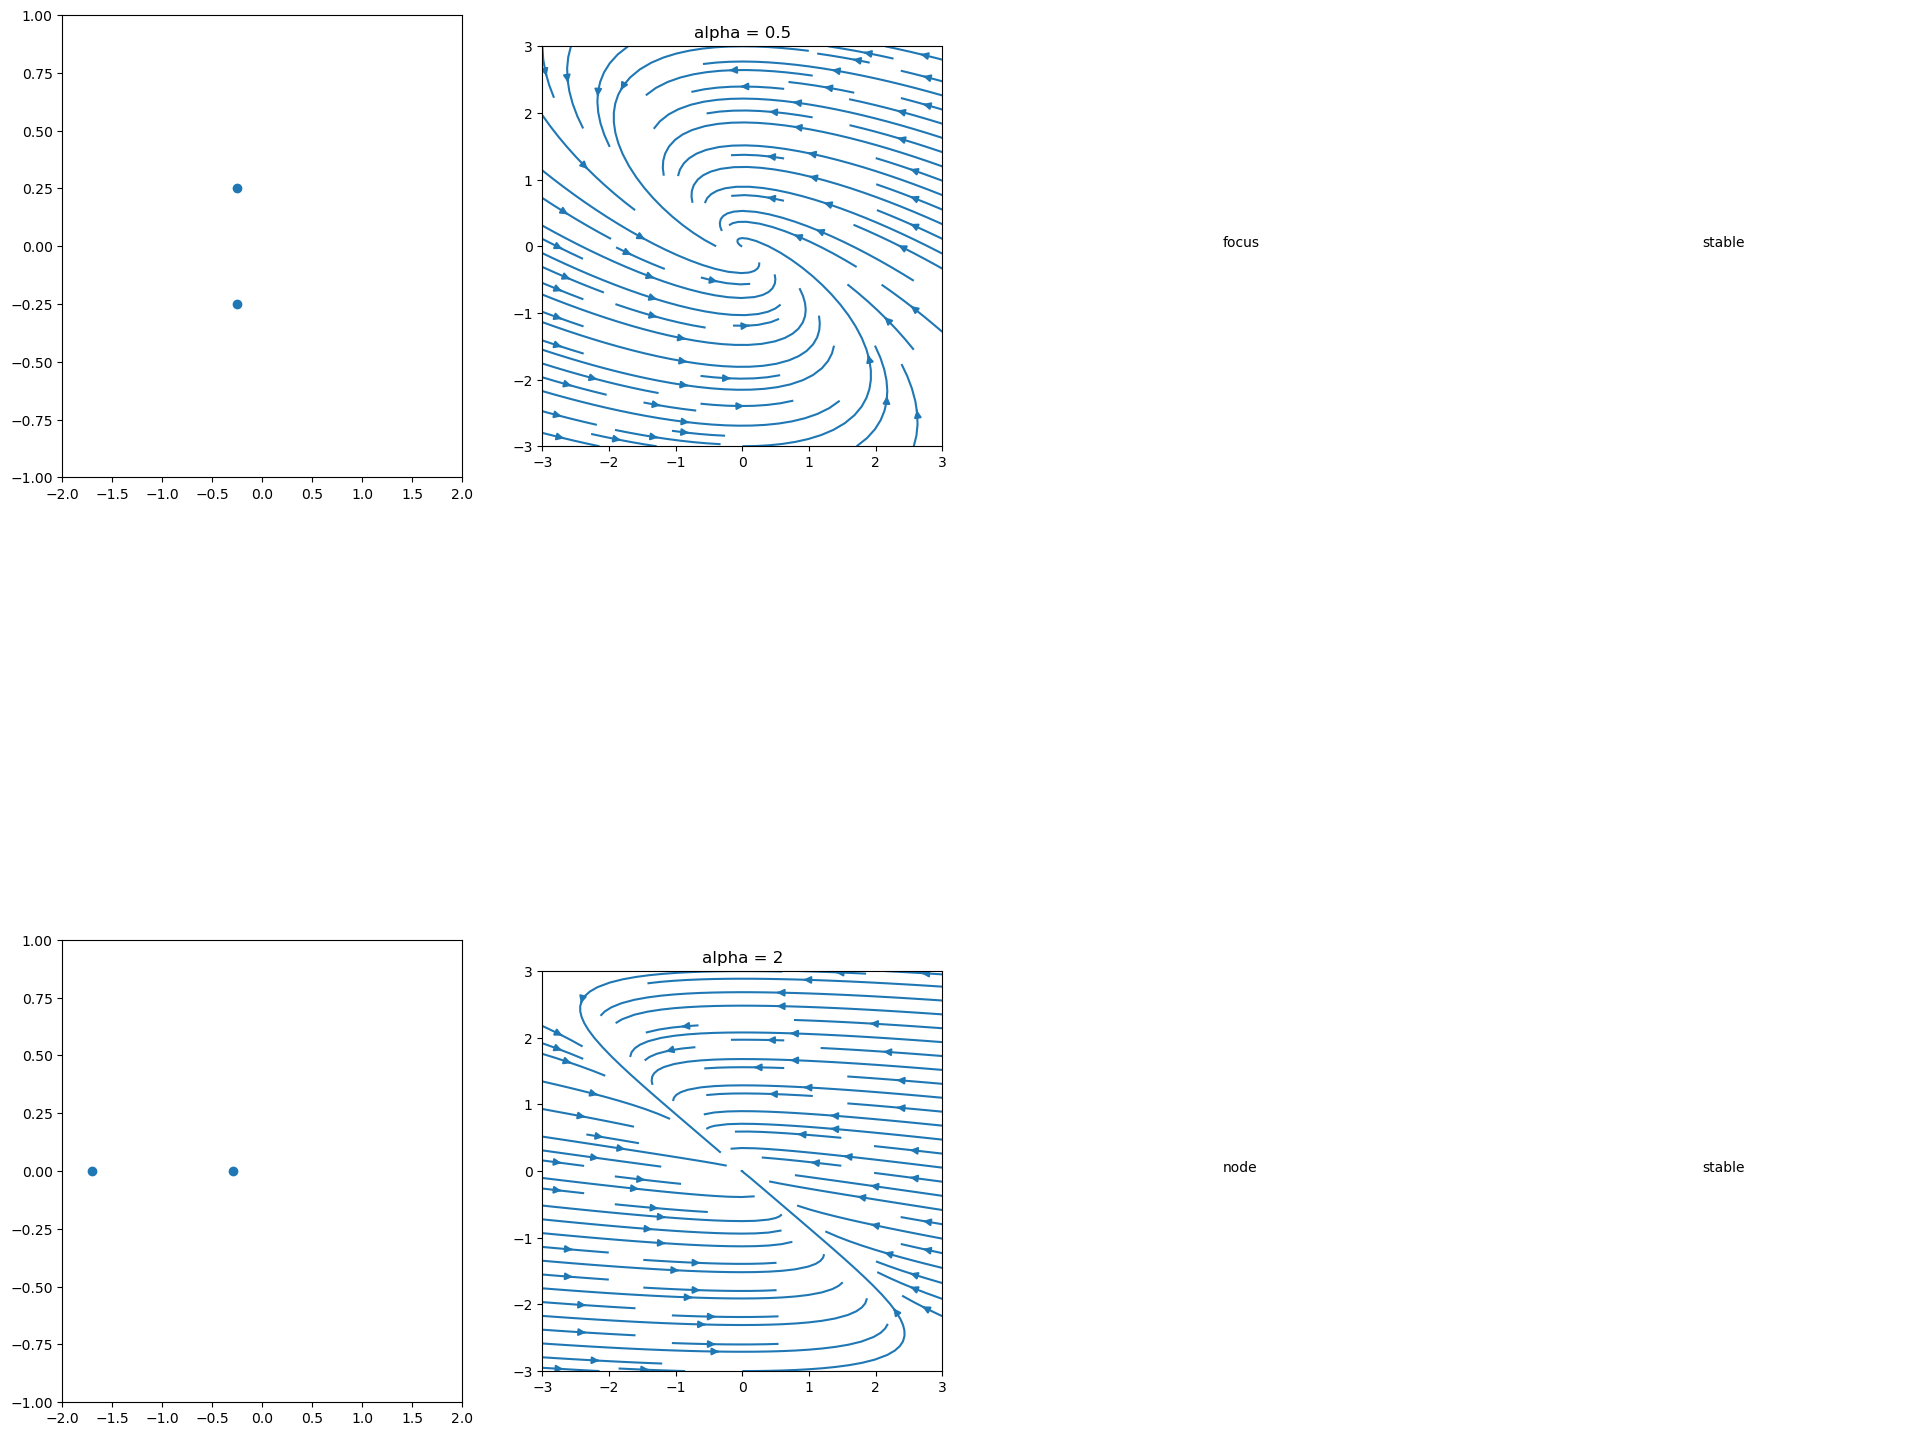
\includegraphics[width=0.5\textwidth]{images/kuzemu0.png}}
\subfigure[using $A_\alpha$]{
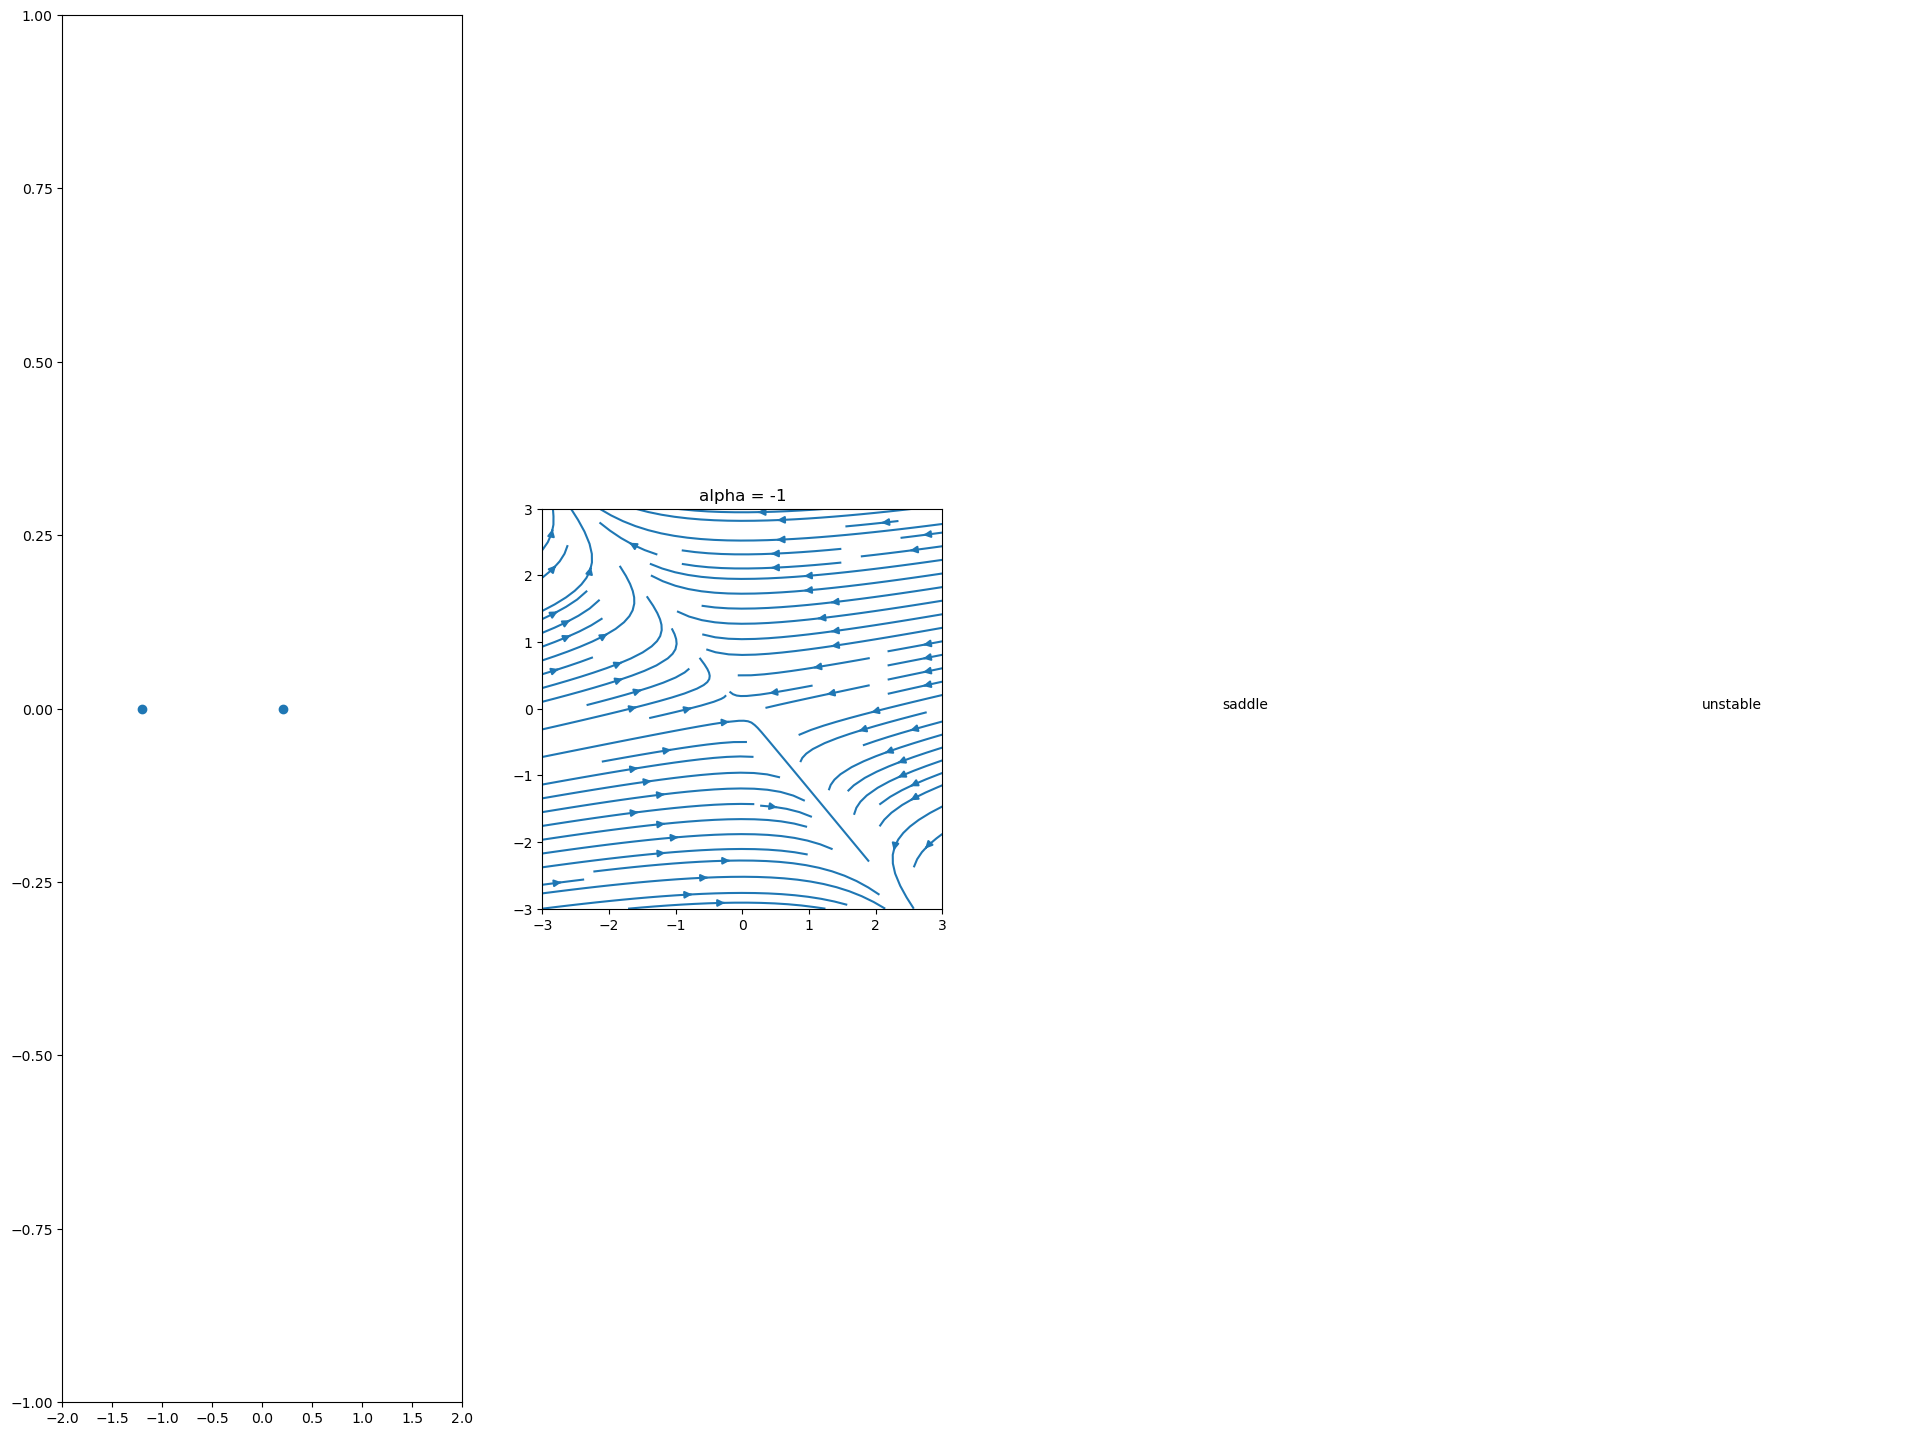
\includegraphics[width=0.5\textwidth]{images/kuzemu1.png}}
\subfigure[using $A_\alpha$]{
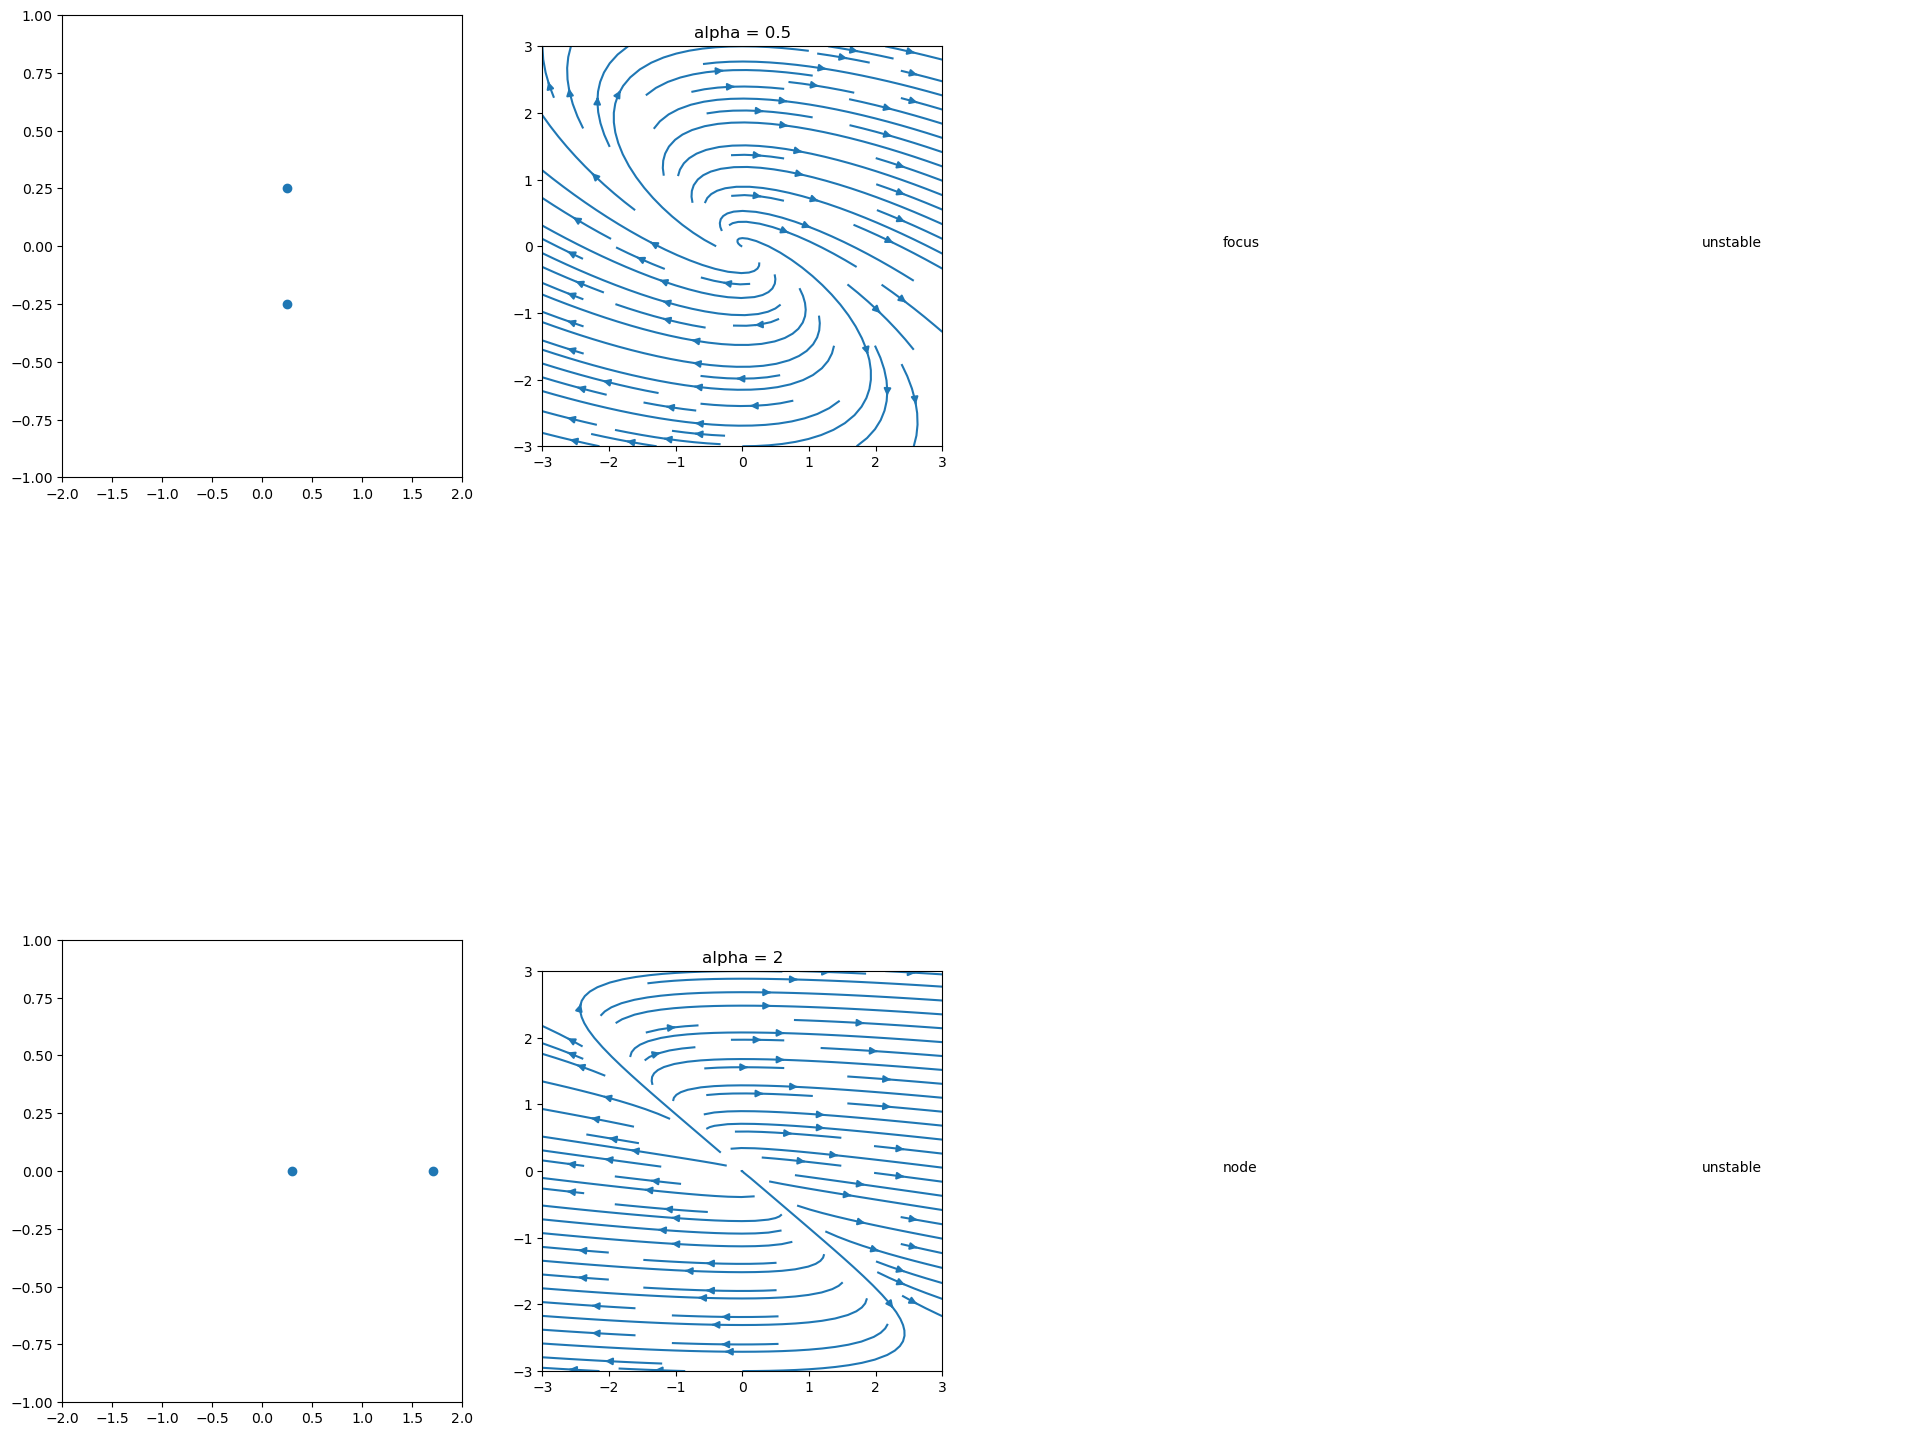
\includegraphics[width=0.5\textwidth]{images/kuzemu2.png}}
\caption{Topological classification of different equilibria on the plane.}
\label{Topological classification}
\end{figure}

Systems with nodes and focus positioned identically and possessing the same stability will be topologically equivalent. In Figure \ref{Topological classification}, this equivalence holds between the first and second systems, as well as between the second-to-last and last systems. However, all other pairs are not topologically equivalent.

\end{task}